{%
\parindent0pt
    \sffamily
    \begin{minipage}[t]{.5\textwidth}
    \vspace{0pt}
    Universit\'e de Lille \\
    \'Ecole Doctorale MADIS \\
    UMR CRIStAL
    \bigskip

    KU Leuven \\
    Groupe des Sciences Biom\'edicales \\
    \'Ecole Doctorale des Sciences Biom\'edicales \\
    Facult\'e des Sciences M\'edicales\\
    D\'epartment des Neurosciences

    \end{minipage}\hfill%
    \begin{minipage}[t]{.3\textwidth}
      \vspace{0pt}
      
\includegraphics[width=\textwidth]{figures/ulille.png}
      \smallskip

      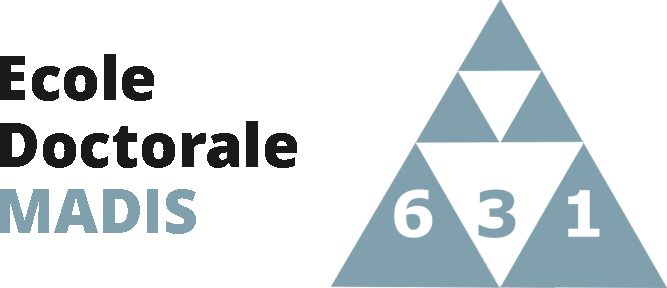
\includegraphics[width=\textwidth]{figures/edmadis.pdf}
      \smallskip


      
\includegraphics[width=\textwidth]{figures/kul.png}
    \end{minipage}

    \vfill

    \makebox[\textwidth][c]{%
      \begin{minipage}{\textwidth}
        \centering
        {%
          \huge
          \bfseries
          Interface Cerveau-Ordinateur visuelle pour la communication sans le regard
        }
        \bigskip

        \MakeUppercase{%
          \Large
          Algorithmes \& Applications
        }
        \bigskip

        {%
          \Large
          Arne  Van Den Kerchove
        }

      \end{minipage}%
    }

    \vfill
      \small
      Th\`ese soutenue le 16 d\'ecembre 2024 en satisfaction partielle des exigences de double
      dipl\^ome de Docteur en Traitement du Signal et des Images
      (Universit\'e de Lille) et Docteur en Sciences Biom\'edicales (KU Leuven)
      devant le jury compos\'e de: \\
      \smallskip

     Pr\'esident: \emph{Prof.\ Koen Poesen, KU Leuven, D\'epartment des Neurosciences} \\
      Rapporteuse: \emph{Prof.\ Andrea K\"ubler, Univ. W\"urzburg, Institut de Psychologie} \\
      Rapporteur: \emph{Prof.\ Fabien Lotte, Inria Bordeaux, LaBRI} \\
      Rapporteur: \emph{Prof.\ Reinhold Scherer, Univ. Essex, École d'informatique et de G\'enie \'Electronique} \\
      Examinateur: \emph{Prof.\ Maarten De Vos, KU Leuven,  D\'epartment de G\'enie \'Electrique} \\
      Examinateur: \emph{Prof.\ Adalberto Simeone, KU Leuven, D\'epartment d'Informatique} \\
      Co-directeur de th\`ese (invit\'e): \emph{Prof.\ François Cabestaing, Univ. Lille, UMR CRIStAL} \\
      Co-directeur de th\`ese (invit\'e): \emph{Prof.\ Marc Van Hulle, KU Leuven, D\'epartment des Neurosciences}

}
